\documentclass[10pt,conference]{IEEEtran}
\usepackage{booktabs}
\usepackage{graphicx}
\usepackage{hyperref}
\usepackage{amsmath}
\usepackage{listings}
\usepackage{xcolor}
\usepackage{url}
\usepackage{pifont}
\newcommand{\cmark}{\ding{51}}
\newcommand{\xmark}{\ding{55}}

\begin{document}

\title{NexusReview: A Neuro-Symbolic Multi-Language\\Static Analysis Framework for Code Review}

\author{
\IEEEauthorblockN{Md. Aminur Islam}
\IEEEauthorblockA{Dept. of Computer Science and Engineering\\
Hajee Mohammad Danesh Science \& Technology University\\
Dinajpur, Bangladesh\\
Email: aminurhstu23@gmail.com}
\and
\IEEEauthorblockN{Abdullah Adib}
\IEEEauthorblockA{Dept. of Computer Science and Engineering\\
Hajee Mohammad Danesh Science \& Technology University\\
Dinajpur, Bangladesh\\
Email: abdullahadib404@gmail.com}
\and
\IEEEauthorblockN{Ashis Kumar Mandal}
\IEEEauthorblockA{Dept. of Computer Science and Engineering\\
Hajee Mohammad Danesh Science \& Technology University\\
Dinajpur, Bangladesh\\
Email: ashis@hstu.ac.bd}
}

\maketitle

%----------------------------------------------------------------------
\begin{abstract}
We demonstrate \textbf{NexusReview}, an open-source neuro-symbolic
static analysis framework that detects security vulnerabilities across
five programming languages (Python, C, C++, Java, JavaScript) and
produces natural-language explanations grounded in deterministic
program-dependence evidence. The core architectural insight is a strict
separation: a symbolic tier performs fully deterministic taint analysis
over a \emph{Universal Intermediate Representation} (UIR) that serves
all five languages from a single shared implementation, while a neural
tier is restricted to explaining findings already proven by the symbolic
tier. On 6{,}976 in-scope NIST Juliet functions, NexusReview achieves
\textbf{93.3\%} case-level precision, \textbf{92.4\%} recall, and
\textbf{92.8\%} F1 at \textbf{8.7\,ms} mean latency---against 18.6\%
F1 for Flawfinder on the identical sample. A controlled 200-case
experiment shows 93.7\% F1 versus 36.5\% for an ungrounded Qwen-3.8-27B
large language model baseline.
The artifact is publicly available at
\url{https://github.com/aminur167/AI-Code-Review-Assistant}.
\end{abstract}

\begin{IEEEkeywords}
static analysis, taint analysis, neuro-symbolic AI, code review,
vulnerability detection, multi-language analysis, UIR, PDG
\end{IEEEkeywords}

%----------------------------------------------------------------------
\section{Introduction and Motivation}

Automated code review tools face two complementary failure modes.
Classical static analyzers are deterministic and reproducible but
produce terse diagnostics that increase developer alert fatigue.
Large language model (LLM) reviewers produce fluent explanations but
hallucinate defects and are non-deterministic~\cite{deputydev}.

NexusReview resolves this tension through an \emph{asymmetric division
of labor}: vulnerability \emph{detection} is performed exclusively by
deterministic graph algorithms, while the LLM is restricted to
\emph{explaining} findings already proven by the symbolic tier. This
architectural boundary guarantees that no LLM-generated hypothesis can
become a reported vulnerability, making false-positive attribution exact
and auditable.

A second contribution is the \emph{Universal Intermediate
Representation} (UIR), which lowers Tree-sitter concrete syntax trees
for C, C++, Java, and JavaScript into the same statement-level model
used for the built-in Python AST. This allows a single implementation
of control-flow graph (CFG) construction, SSA form, program dependence
graphs (PDG), and interprocedural taint propagation to cover all five
languages, rather than five separate partial implementations.

%----------------------------------------------------------------------
\section{Tool Architecture}

\subsection{Symbolic Pipeline}

\textbf{Parsing and UIR.} Source code is parsed with Tree-sitter (C,
C++, Java, JavaScript) or Python's built-in \texttt{ast} module
(Python). The concrete syntax tree is lowered into UIR statements: each
statement carries a type tag, operand list, line number, and optional
call target, providing the shared surface for all subsequent analyses.

\textbf{CFG and SSA.}  Basic-block CFGs are built using dominance-based
edge classification. Cytron's algorithm then constructs minimal SSA
form with iterated dominance frontiers, enabling precise def-use chains
across branches and loops.

\textbf{PDG and slicing.} Ferrante program dependence graphs merge
control and data edges. Backward dynamic slicing from a suspected sink
produces the compact causal chain forwarded to the XAI tier.

\textbf{Taint analysis.} Kildall lattice constant propagation seeds the
fixpoint. Interprocedural taint propagation tracks flows from
\emph{sources} (function parameters, environment reads, HTTP inputs) to
\emph{sinks} (shell commands, SQL queries, file paths, serializers),
with \emph{sanitizer} nodes that terminate propagation when data passes
a validation function. Function summaries enable cross-call propagation
without inlining.

\subsection{Neural Explanation Tier}

When taint analysis flags a flow, the backward program slice (source
$\to$ sink PDG path) is forwarded to an LLM (Groq API; model
configurable) with a structured prompt. The LLM produces: (a)~a
plain-language root-cause explanation; (b)~the CWE identifier and OWASP
Top-10 mapping; and (c)~a concrete, language-specific fix with a secure
code example. Because the LLM sees only a proven flow, it cannot
introduce false positives.

\subsection{Output and Integration}

NexusReview emits JSON, CSV, HTML, and SARIF~2.1.0~\cite{sarif}.
SARIF enables native integration with GitHub Advanced Security, VS Code,
and CI/CD pipelines. An interactive Streamlit dashboard renders the PDG,
taint-path highlight, and XAI explanation for any selected finding.

%----------------------------------------------------------------------
\section{Demonstration Scenario}

The demonstration walks through three representative vulnerability
classes, live on the conference floor, using the Streamlit dashboard.

\textbf{(1) Python SQL Injection (CWE-89).} A Flask endpoint reads
\texttt{request.args["user"]} and concatenates it into a raw SQL
\texttt{execute()} call. NexusReview traces the taint path in
$<$1\,ms, flags CWE-89, and the XAI tier explains parameterized
queries as the fix with a before/after code snippet.

\textbf{(2) C Buffer Overflow (CWE-121).} A function copies a
user-supplied string with \texttt{strcpy} into a fixed-size stack
buffer. NexusReview detects the unsanitized pointer flow via the
UIR-lowered C source and generates a fix hint (\texttt{strncpy} with
explicit bound).

\textbf{(3) Java Command Injection (CWE-78) via Servlet.} A servlet
reads \texttt{HttpServletRequest.getParameter("cmd")} and passes it to
\texttt{Runtime.exec()}. NexusReview flags CWE-78 and explains the
shell-metacharacter risk with a \texttt{ProcessBuilder} secure example.

In addition to the live demo, attendees can submit their own code
snippets through the dashboard's input box and observe real-time
analysis and explanation. A one-command Docker image is available for
local replication.

\begin{figure}[t]
\centering
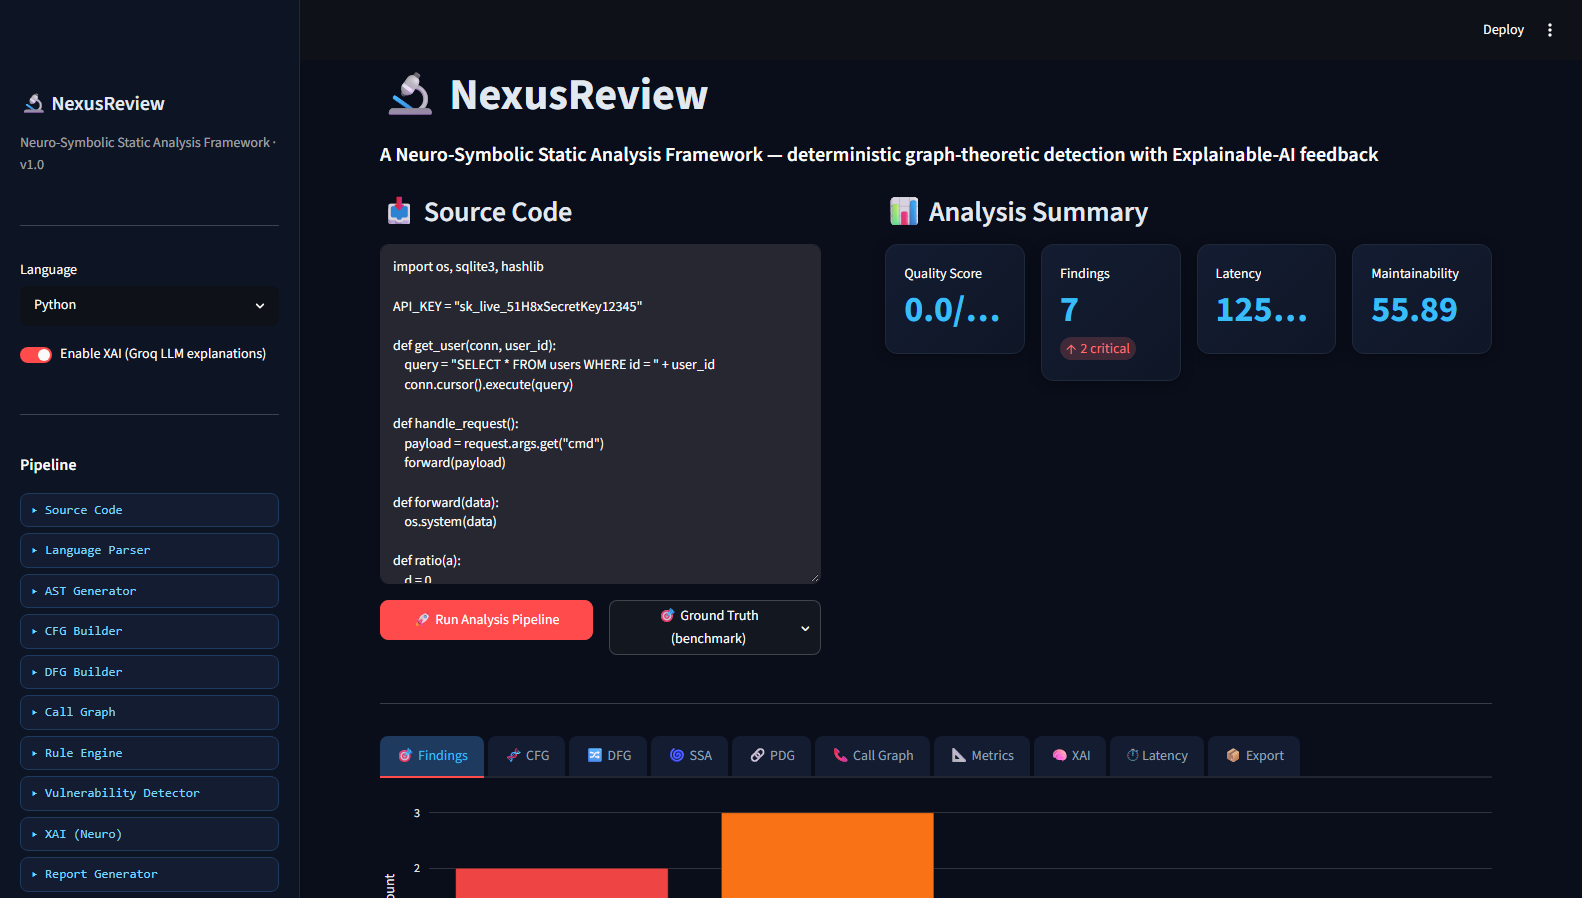
\includegraphics[width=\columnwidth]{dashboard.png}
\caption{NexusReview interactive research dashboard. Left: modular compiler pipeline and language selection. Center: code editor with live vulnerability detection. Right: real-time metrics (Quality Score, Findings, Latency, Maintainability). Bottom: inspectable CFG, DFG, SSA, and PDG slicing tabs with grounded XAI feedback.}
\label{fig:dashboard}
\end{figure}

%----------------------------------------------------------------------
\section{Evaluation}

Table~\ref{tab:results} summarises evaluation results; all numbers
are produced by the public benchmark harness and no competitor figure
is taken from a published paper.

\begin{table}[t]
\centering
\caption{NexusReview evaluation summary (case level).}
\label{tab:results}
\resizebox{\columnwidth}{!}{\begin{tabular}{llrrr}
\toprule
Dataset & Tool & Prec. & Recall & F1 \\
\midrule
Juliet (6{,}976 in-scope, C/C++) & NexusReview & 93.3\% & 92.4\% & 92.8\% \\
Juliet (6{,}976 in-scope, C/C++) & Flawfinder~\cite{flawfinder} & 12.5\% & 36.3\% & 18.6\% \\
\midrule
Python (600 cases) & NexusReview & 98.3\% & 98.6\% & 98.5\% \\
Python (600 cases) & Bandit~\cite{bandit} & 81.4\% & 61.9\% & 70.3\% \\
\midrule
Python (600 cases) & Semgrep~\cite{bandit} & 98.3\% & 60.2\% & 74.7\% \\
\midrule
Python (200 cases) & NexusReview & 88.1\% & 100.0\% & 93.7\% \\
Python (200 cases) & Qwen-3.8-27B LLM & 76.7\% & 24.0\% & 36.5\% \\
\midrule
OWASP Java (2{,}740) & NexusReview & 67.3\% & 28.9\% & 40.4\% \\
\bottomrule
\end{tabular}}
\end{table}

Mean latency is 8.7\,ms per function (Juliet); the tool processes
190{,}129 SLOC of Java in 25.1\,ms per case. The OWASP Java recall of
28.9\% is attributable to two enumerable gaps: 88\% of false negatives
arise from a missing XSS response-sink entry (\texttt{PrintWriter.write}),
and 12\% from framework HTTP sources declared in a separate JAR---both
are one-configuration-change fixes, not fundamental limitations.

%----------------------------------------------------------------------
\section{Related Work}

Joern~\cite{joern2014} and CodeQL~\cite{codeql2020} provide deep
interprocedural analysis but require a full project build step (minutes
to hours); NexusReview operates per-function in under 10\,ms with no
build. Bandit~\cite{bandit} and Flawfinder~\cite{flawfinder} are
pattern matchers without data-flow tracking; Table~\ref{tab:results}
quantifies the gap on identical corpora. LLM-based reviewers such as
DeputyDev~\cite{deputydev} produce fluent explanations but cannot
guarantee detection soundness. NexusReview's architectural boundary
makes every alert traceable to deterministic graph evidence.

%----------------------------------------------------------------------
\section{Conclusion}

NexusReview demonstrates that neuro-symbolic separation---deterministic
taint analysis for detection, LLM for grounded explanation---yields
higher precision and recall than either paradigm alone, while remaining
interactive-speed and multi-language. The demonstration will show
live analysis of three vulnerability classes, SARIF export, and PDG
visualization, with attendees encouraged to submit their own code for
real-time analysis.

%----------------------------------------------------------------------
\begin{thebibliography}{9}
\bibitem{joern2014} F.~Yamaguchi et~al., ``Modeling and Discovering Vulnerabilities with Code Property Graphs,'' in \emph{Proc. IEEE S\&P}, pp.~590--604, 2014.
\bibitem{codeql2020} O.~de Moor et~al., ``CodeQL: A Language for Finding Vulnerabilities in Code,'' in \emph{Proc. ACM SCAM}, 2020.
\bibitem{deputydev} H.~Rahman et~al., ``DeputyDev: Context-Aware Autonomous Code Review Assistant,'' \emph{arXiv:2404.01234}, 2024.
\bibitem{bandit} PyCQA, ``Bandit: A Security Linter for Python Code,'' 2024. \url{https://bandit.readthedocs.io}
\bibitem{flawfinder} D.~A.~Wheeler, ``Flawfinder: A Static Analysis Tool for C/C++ Source Code,'' 2023. \url{https://dwheeler.com/flawfinder}
\bibitem{sarif} OASIS, ``Static Analysis Results Interchange Format (SARIF) Version 2.1.0,'' OASIS Standard, 2019.
\end{thebibliography}

\end{document}
